\documentclass{aastex62}
\submitjournal{ApJS}
\shorttitle{A reference transient dataset I: lightcurves}
\shortauthors{Neira et al.}

\usepackage{import}
\usepackage{hyperref}
\usepackage[T1]{fontenc}

\usepackage{graphicx}
\usepackage{amsmath}
\usepackage{amssymb}

\usepackage[utf8]{inputenc}
\usepackage{multirow}
\usepackage{float} 

\begin{document}
\title{A eference dataset for astronomical transient event recognition I: lightcurves}

\author{Mauricio Neira}
\affiliation{
Systems and Computing Engineering Department\\
Universidad de los Andes\\
Cra. 1 No. 18A-10\\
Bogot\'a, Colombia}

\author{Catalina G\'omez}
\affiliation{Departamento de Ingenier\'ia Biom\'edica\\
Universidad de los Andes\\ 
Cra. 1 No. 18A-10\\
Bogot\'a, Colombia\\}

\author{Diego A. G\'omez}
\affiliation{
Systems and Computing Engineering Department\\
Universidad de los Andes\\
Cra. 1 No. 18A-10\\
Bogot\'a, Colombia}

\author{Juan Pablo Reyes}
\affiliation{
Systems and Computing Engineering Department\\
Universidad de los Andes\\
Cra. 1 No. 18A-10\\
Bogot\'a, Colombia}

\author{Marcela Hern\'andez Hoyos}
\affiliation{
Systems and Computing Engineering Department\\
Universidad de los Andes\\
Cra. 1 No. 18A-10\\
Bogot\'a, Colombia}


\author{Pablo Arbel\'aez}
\affiliation{Departamento de Ingenier\'ia Biom\'edica\\
Universidad de los Andes\\ 
Cra. 1 No. 18A-10\\
Bogot\'a, Colombia}

\author{Jaime E. Forero-Romero}
\affiliation{Departamento de F\'isica\\
Universidad de los Andes\\
Cra. 1 No. 18A-10\\
Bogot\'a, Colombia}


\begin{abstract}
We introduce ATTAC (Annotated Transient caTAlina Catalog) an
annotated dataset of $4869$ transient and $16940$ non-transient
object lightcurves built from the Catalina Real Time Transient
Survey.
We provide public access to this dataset as a plain text file to facilitate
standardized quantitative comparison of astronomical transient event
recognition algorithms. 
Some of the classes included in the dataset are: supernovae, cataclismic
variables, active galactic nuclei, high proper motion stars, blazars
and flares.
As a complement to the dataset, we experiment with multiple
data pre-processing methods, feature selection techniques and popular
machine learning algorithms (Support Vector Machines, Random Forests
and Neural Networks).   
We assess quantitative performance in two classification tasks:
binary (transient/non-transient) and eight-class classification.   
The best performing algorithm is a Random Forest Classifier for both
classification experiments.  
The next release of ATTAC will include images and benchmarks with
deep learning models. 
\end{abstract}

\keywords{catalogs}

\section{Introduction}



Large scale automatic detection and classification of astronomical
transients is happening within surveys such as Pan-STARRS1
\citep{2004SPIE.5489...11K}, the Palomar Transient Factory
\citep{2009PASP..121.1395L},  the Catalina Real-Time Transient Survey
\citep{2009ApJ...696..870D}, the All-Sky Automated Survey for
SuperNovae \citep{2014ApJ...788...48S}, the Zwicky Transient
Factory \citep{2019PASP..131a8002B}.
Besides the large amount of data, transient
classification is hard because the data is usually heterogeneous,
unbalanced, sparse, unevenly sampled and with missing information.   

These two characteristics (size and heterogeneity) have
motivated the application of Machine Learning (ML) algorithms to face
this challenge.  
For instance, Random Forests, MultiLayer Perceptron and K-Nearest
Neighbours have been used on lightcurves to classify transients from
the Catalina Real Time Transient Survey \citep{1601.03931};  
convolutional neural networks have been used as 
input to automatic vetting algorithms (quick classification of bogus
vs. real transients) based on data from the SkyMapper Supernova and
Transient  Survey and the High cadence Transient Survey (HiTS)
\citep{1708.08947,1701.00458}.

The success of these examples, and any other ML implementation,
depends on the quality of the training dataset.
New ML results usually come from groups internal to an observational
collaboration because they have the internal know-how (and, sometimes,
privileged access) to experiment and build training datasets.
This difference in data access, makes it challenging for other
scientists to rebuild a training dataset, perform comparisons with
published results and suggest new algorithms. 

Nonetheless, building traning datasets has been facilitated by the
publication of large databases from different observational projects.
Other collaborations have directly published large datasets of simulated
hoping to trigger more involvement from the ML in astronomy
community at large to develop new classification algorithms \citep{2018arXiv181000001T}.

In this paper we aim at bridging the data access gap.
We compile and publish in easy-to-access files a dataset
that can be used to train and test different ML algorithms for
transient detection. 
We use public data from the Catalina Real-Time Transient Survey
(CRTS) \citep{1111.2566}, an astronomical survey searching transient
and highly variable objects as base for the dataset.
Here, in the first paper, we present the lightcurve data.
In a second paper, we will present an imaging dataset from the same
survey.   

\newpage
In Section \ref{sec:data} we present the CRTS and the steps we follow
to build the dataset.
Then, in Section \ref{sec:repository} we describe its main features together
with the repository structure gathering the files and Python code to explore it. 
In Section \ref{sec:ml_tests} we show how this dataset can be used to 
perform tests using ML methods following a similar approach as \cite{1601.03931},
and the experiments that we perform. 
We finalize in Section \ref{sec:conclusions} with a summary of the
main features of our dataset and the results of our experiments. 


\section{The lightcurve dataset} 
\label{sec:data}

We use public data from the Catalina Real-Time Transient Survey
(CRTS) \citep{2009ApJ...696..870D}, an astronomical survey searching transient
and highly variable objects.
The CRTS covered 33000 squared degrees of sky and took data since 2007. 
Three telescopes were used: Mt. Lemmon Survey (MLS), Catalina Sky 
Survey (CSS), and Siding Spring Survey (SSS). So far, CRTS has 
discovered more than $15000$ transient events.
We use data from the CSS telescope, which is an f/1.8 Schmidt
telescope located in the Santa Catalina Mountains in Arizona.
The telescope is equipped with a 111-megapixel  detector, and covered
4000 square degrees per night, with a limiting magnitude of 19.5 in
the V band.  

Putting together the lightcurves for MANTRA implies
cross-matching different files in the legacy CRTS webpage:
\url{http://nesssi.cacr.caltech.edu/DataRelease/CRTS-I_transients.html}. 
The photometry is stored in two different kinds of files: \verb"phot"
that come from the main photometry database and \verb"orphan" that
correspond to transients not associated with the 500 million sources
in the main photometry database.
There are also \verb"out" files that must be used to link transient
IDs to database IDs.


For each one of the 5540 transients reported and classified in the
archival webpage \url{http://nesssi.cacr.caltech.edu/catalina/All.arch.html} we use its
transient IDs and its database IDs to look for the lightcurves in the
\texttt{phot} and \texttt{orphan} files. 
Only 4982 transients can be linked to available data to reconstruct
their lightcurves. 
Furthermore, some of these lightcurves are duplicated, i.e. they had
the same number of observations, Modified Julian Date (MJD) and magnitude measurement. 
We ignore the duplicates to end up with 4869 unique transients with an 
associated lightcurve. Figure \ref{fig:transients} summarizes this process. 

\begin{figure*}
	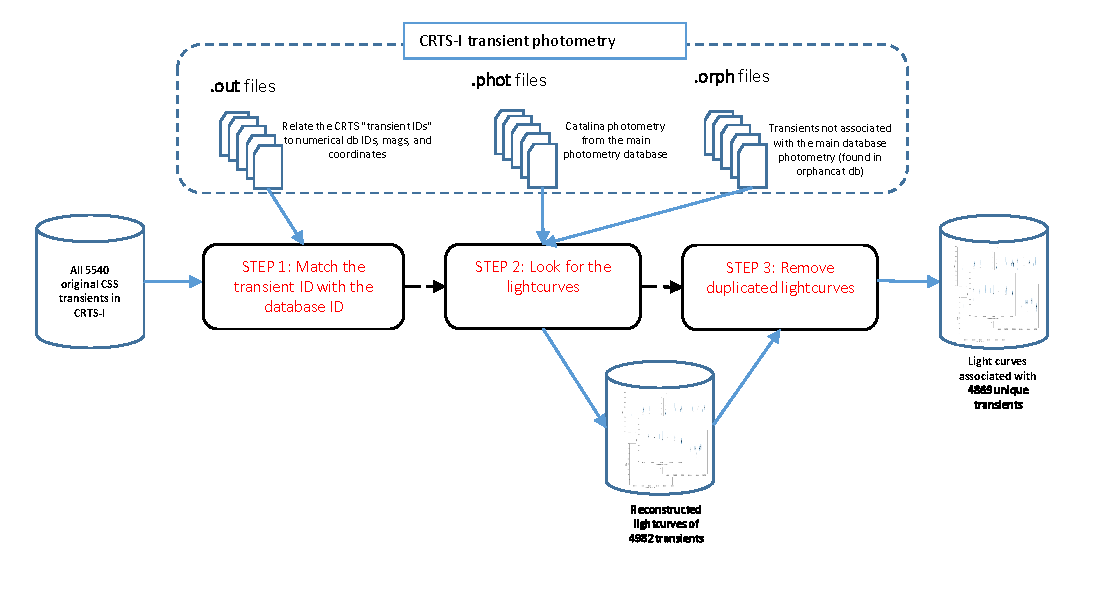
\includegraphics[width=0.9\textwidth]{Transients.pdf}
  \caption{MANTRA Dataset Set Up: Lightcurve compilation for transient classes.}
  \label{fig:transients}
\end{figure*} 

The CRTS dataset already provides a classification. 
The most numerous classes are: supernovae,
cataclysmic variable stars, blazars, flares, asteroids, active
galactic nuclei, and high-proper-motion stars (HPM). 
Though most objects in the transient object catalogue belong to a single class, 
there is some uncertainty in the categorization of some of them.  
In this case, an interrogation sign is used when a class is not clear 
e.g. SN? or sometimes multiple possible classes are found for a single 
event e.g. SN/CV. 
Table \ref{table:top_classes} summarizes the number of objects in each class. 

To compile the non-transient lightcurves we retrieve sources in the
dataset from the CRTS online catalogue by retrieving objects within a
20 arcsecond radius from CRTS detected transients, 
and removing known transient lightcurves from that set. 
We end up with 16940 unique non-transient lightcurves. Figure \ref{fig:non-transients} illustrates this process.

\begin{figure*}
	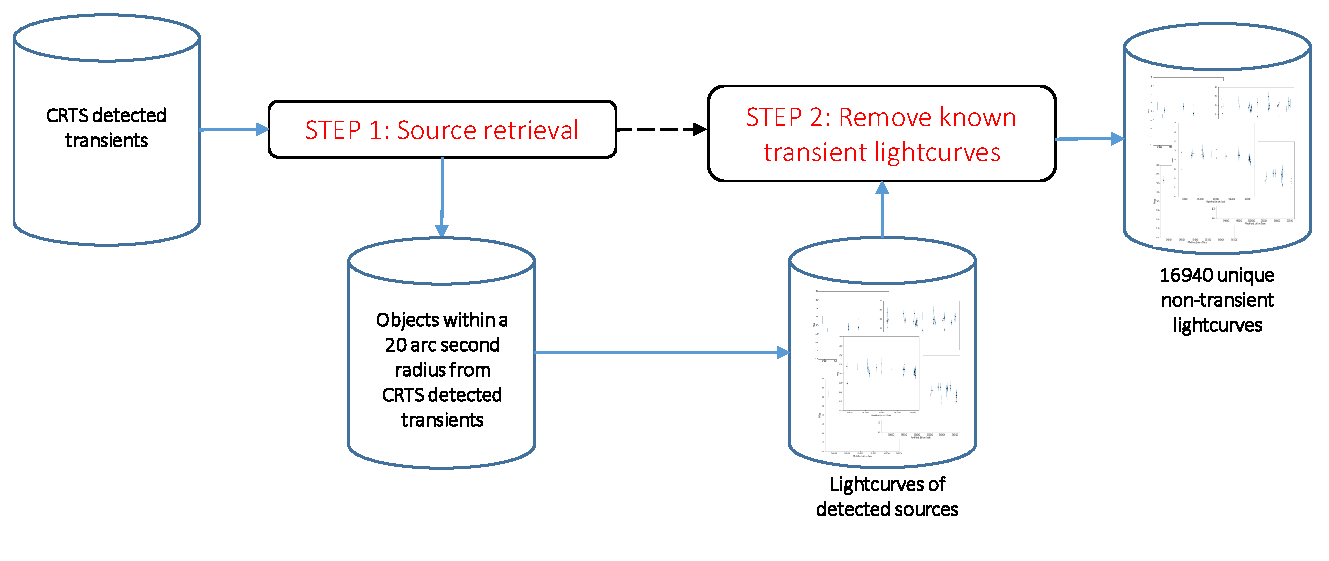
\includegraphics[width=0.7\textwidth]{NonTransients.pdf}
  \caption{MANTRA Dataset Set Up: Lightcurve compilation for non-transients.}
  \label{fig:non-transients}
\end{figure*} 

% Number of transients per transient class
\begin{table}
\centering
\begin{tabular}{c|c}
    \hline
    Class &  Object Count \\
    \hline
SN & 1723 \\
CV & 988 \\
HPM & 640 \\
AGN & 446 \\
SN? & 319 \\
Blazar & 243 \\
Unknown & 228 \\
Flare & 219 \\
AGN? & 138 \\
CV? & 77 \\
    \hline
\end{tabular}
\caption{Top 10 transient classes in the CRTS with their respective number of lightcurves.} 
\label{table:top_classes}
\end{table}


\begin{figure*}
	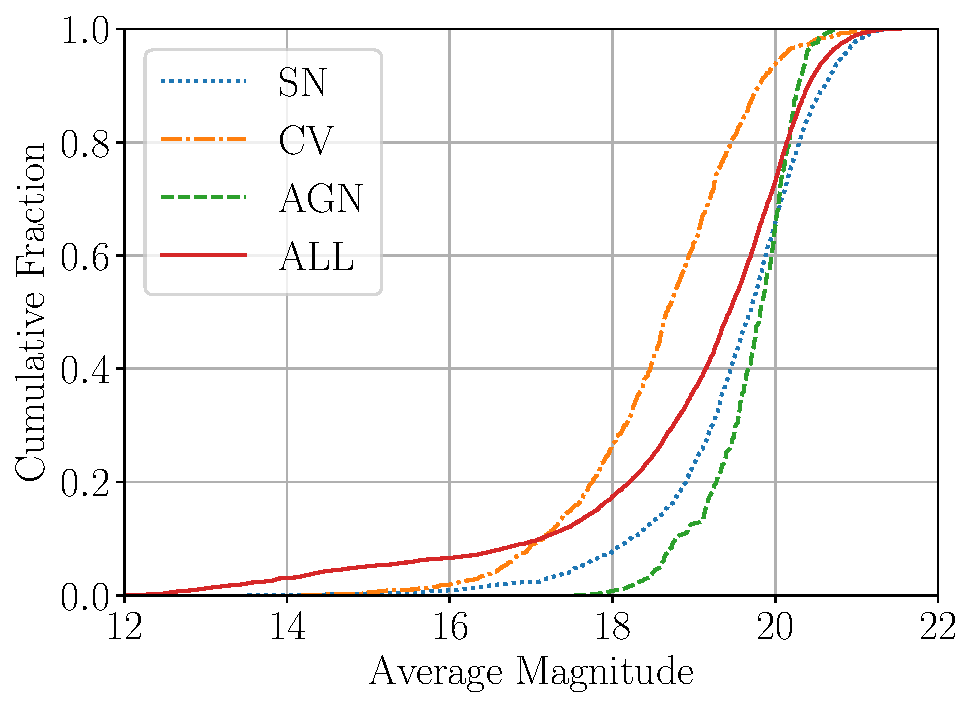
\includegraphics[width=0.45\textwidth]{cumulative_magnitude.pdf}
  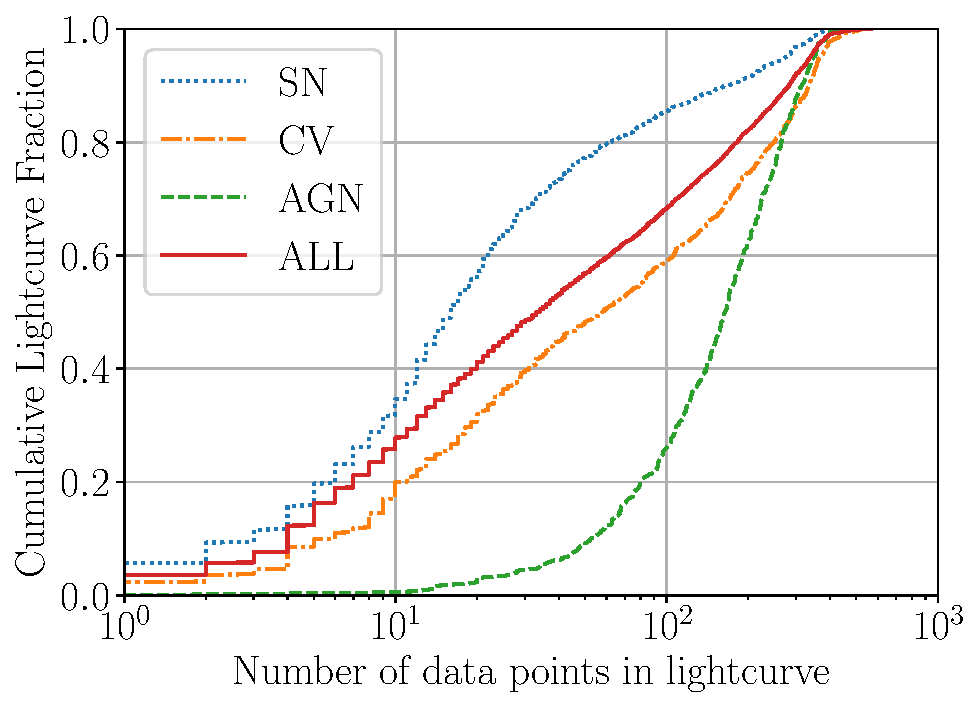
\includegraphics[width=0.45\textwidth]{cumulative_classes.pdf}
  \caption{Cumulative number of lightcurves (expressed as a fraction)
    as a function of average magnitude (left) and number of data
    points in the lightcurve (right).
    This includes information for the three most representative
    classes (SN, CV, AGN) and the whole database (ALL).}
  \label{fig:cumulative}
\end{figure*} 


\begin{figure*}
\begin{center}
  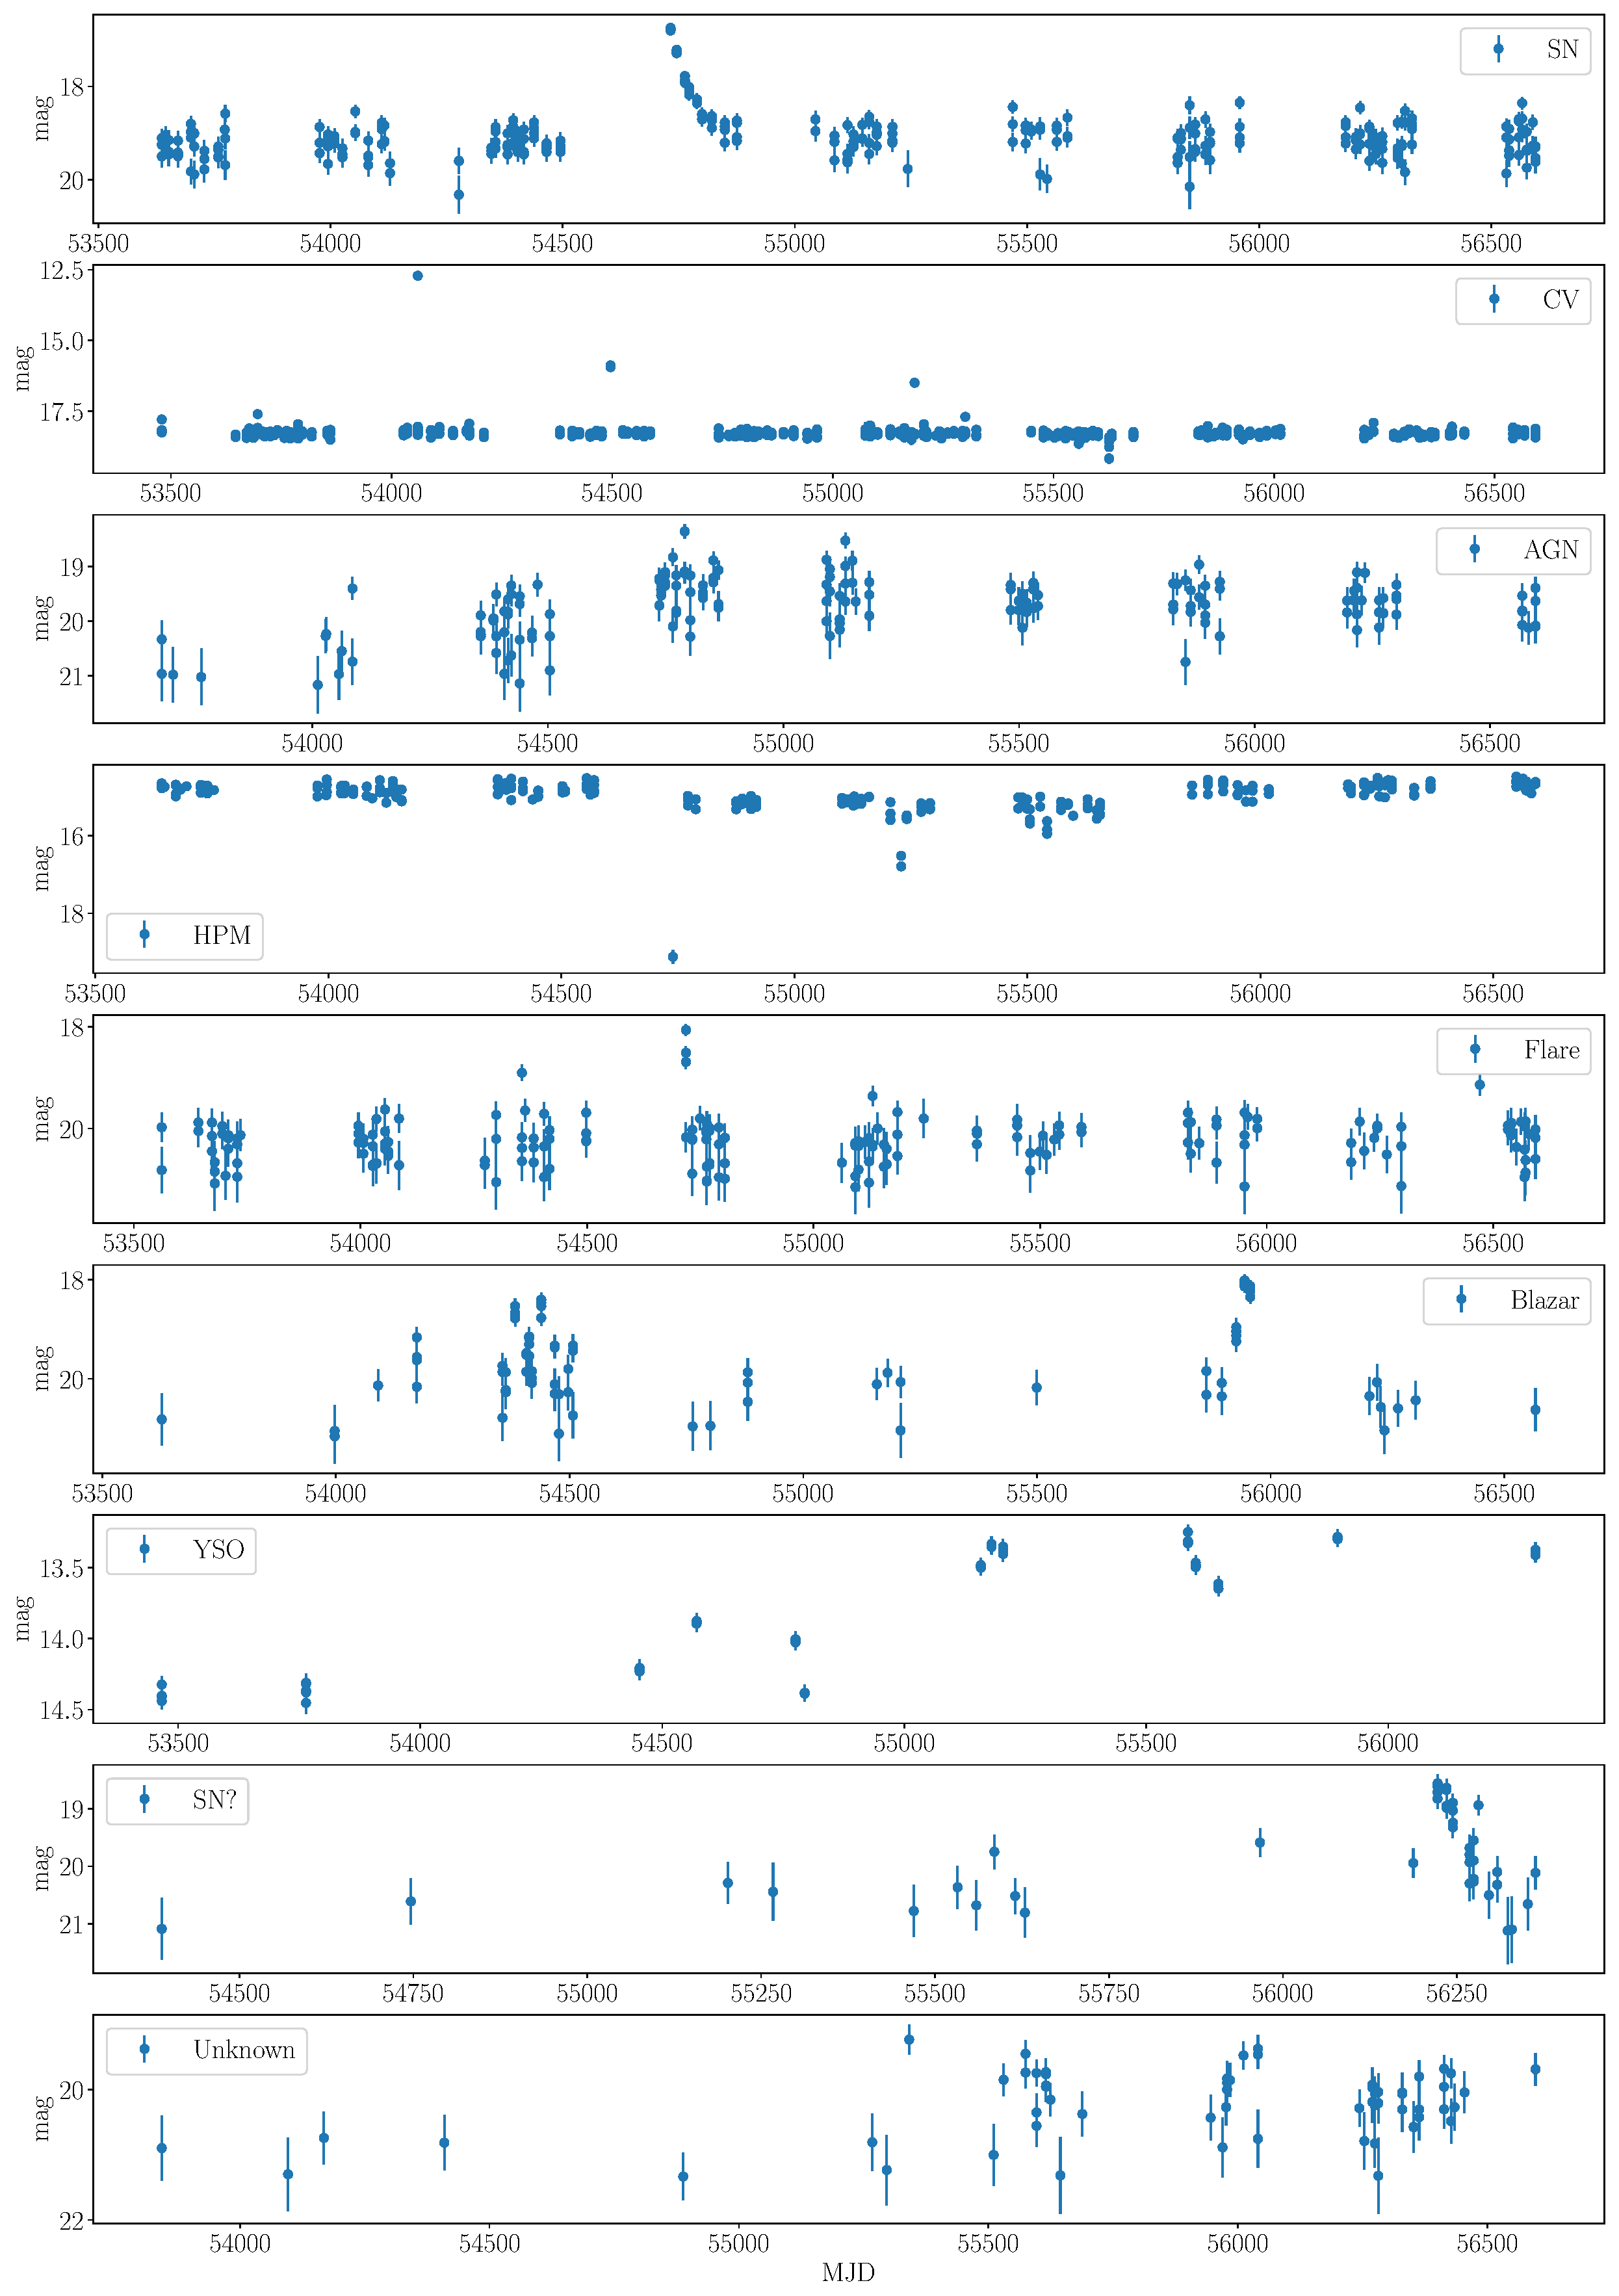
\includegraphics[width=0.6\textwidth]{examples_transient.pdf}
\end{center}
  \caption{Randomly selected lightcurves for the most represented transient classes as compiled in MANTRA. The class of each sample is within the legend box. }  
  \label{fig:examples_transient}
\end{figure*} 


\begin{figure*}
  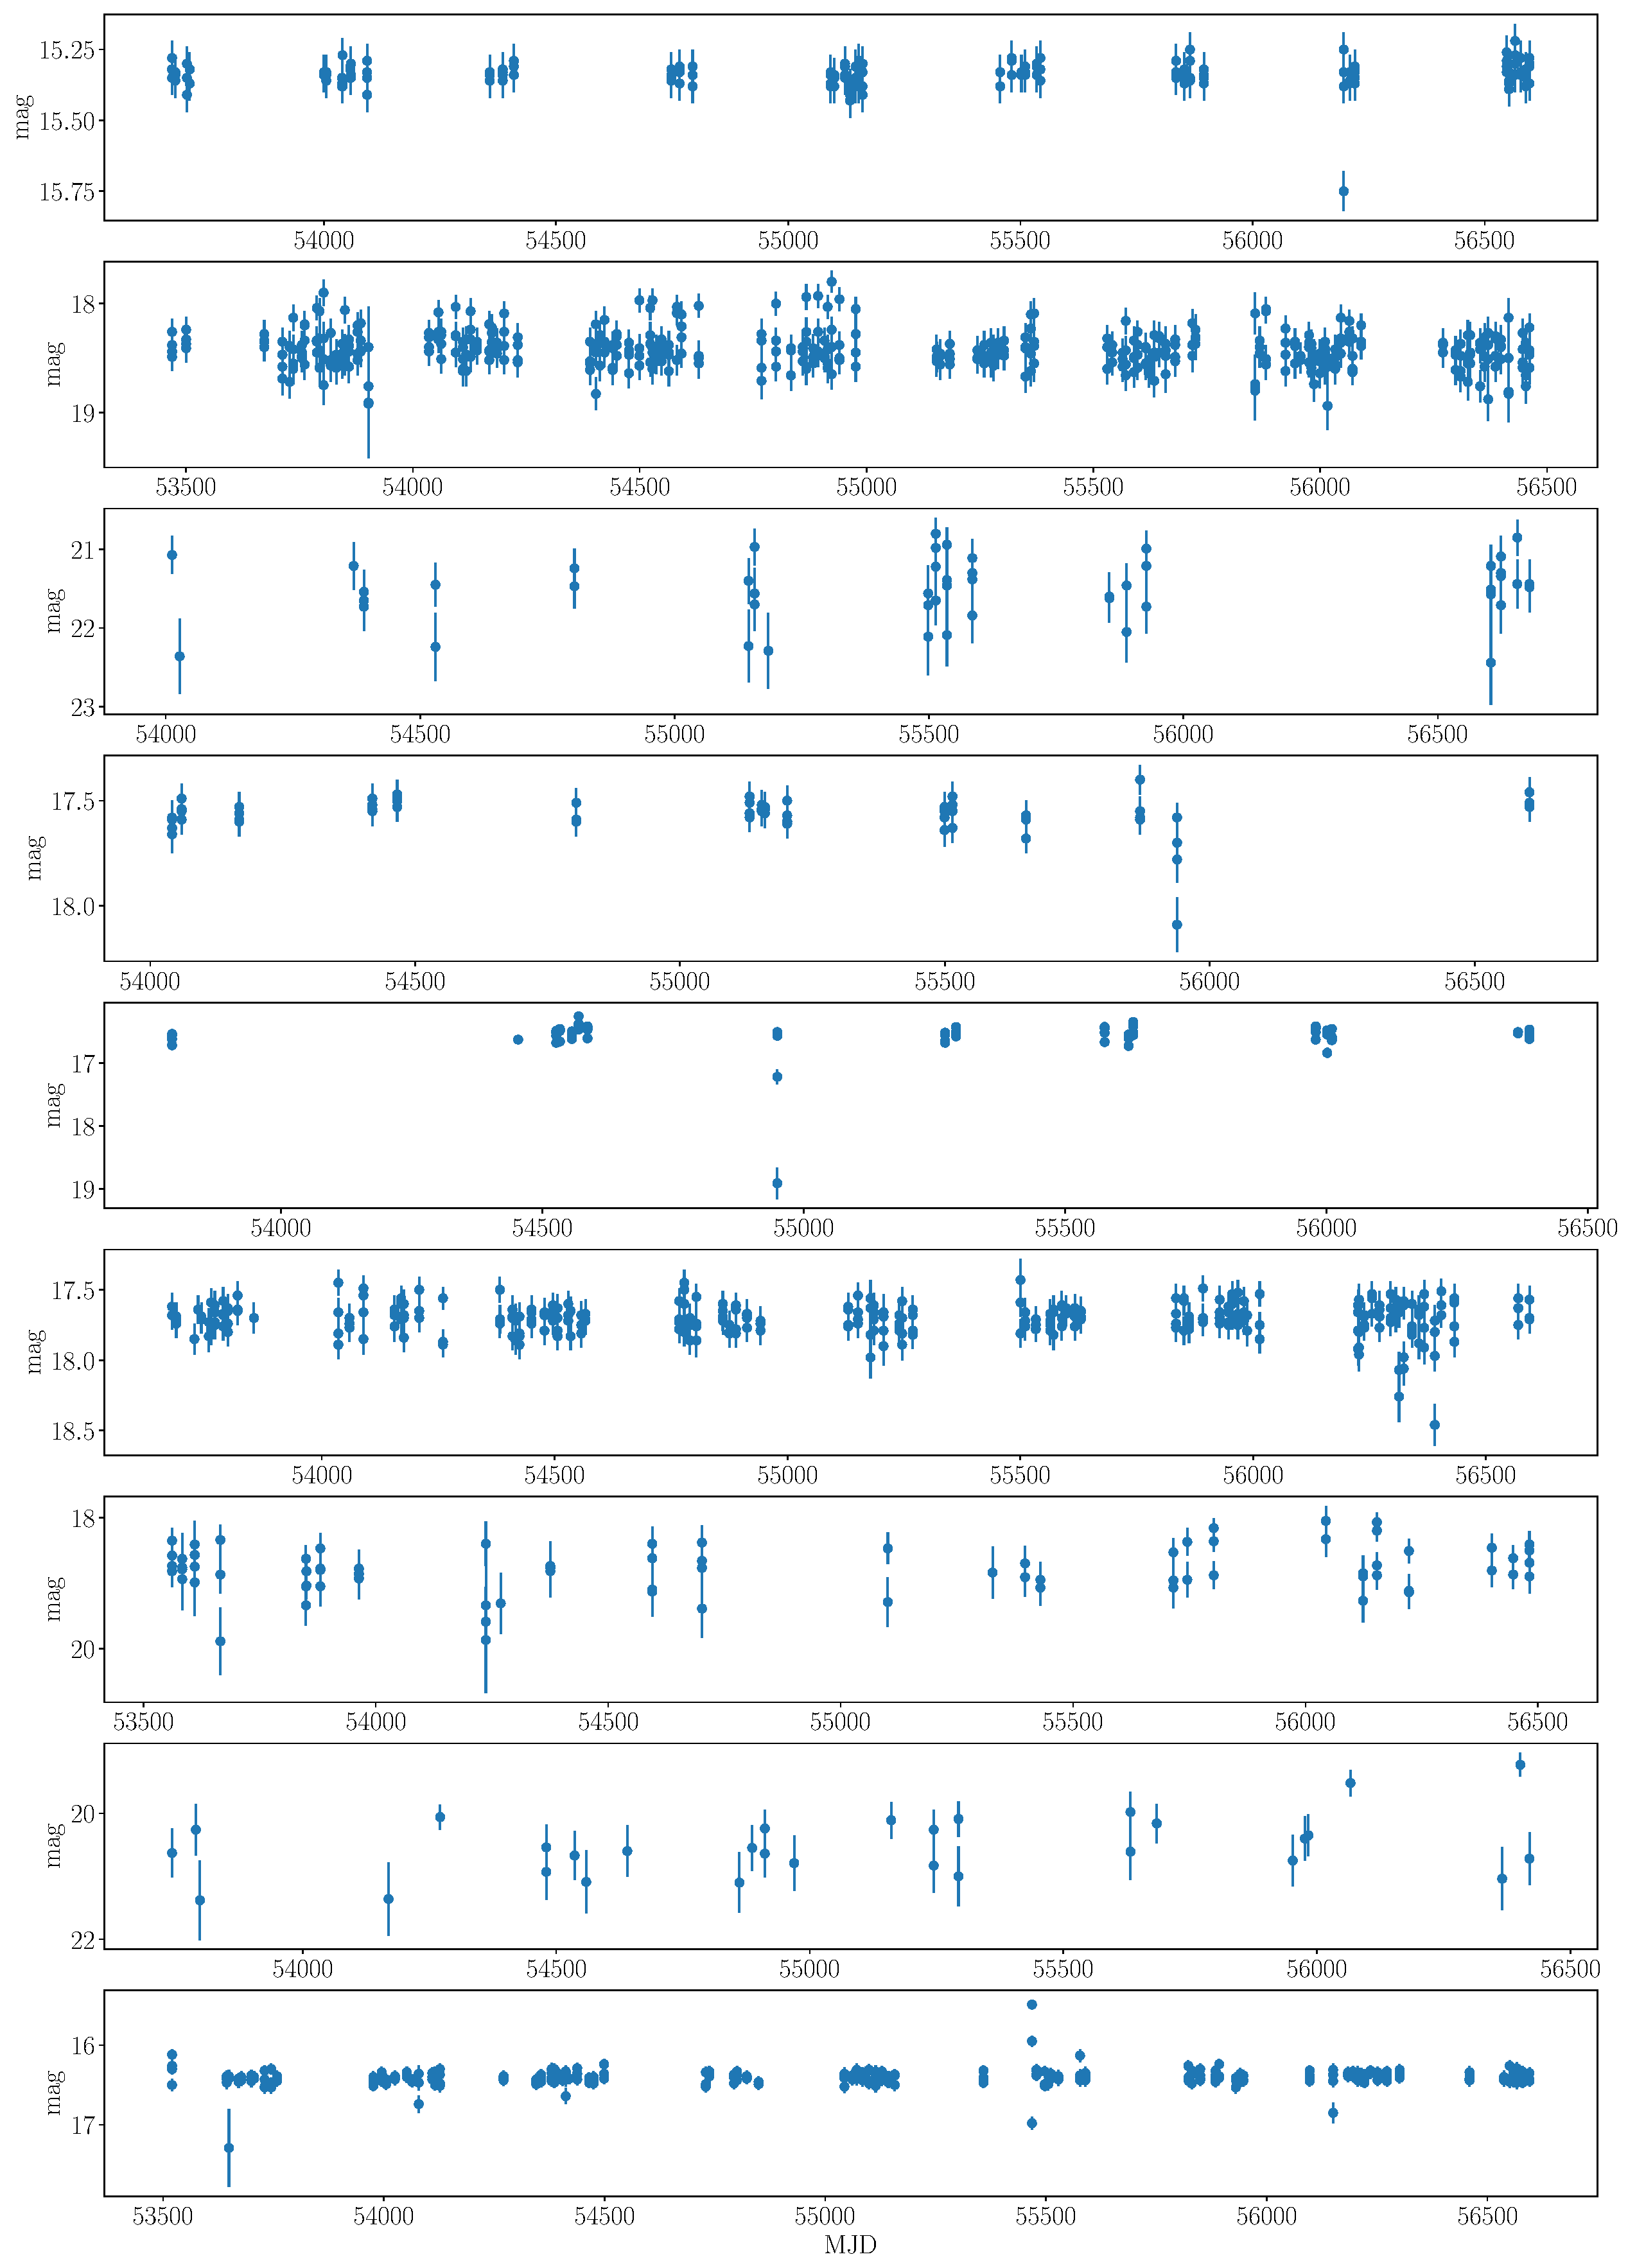
\includegraphics[width=0.6\textwidth]{examples_nontransient.pdf}
  \caption{Randomly selected lightcurves for non-transient sources retrieved for MANTRA.}
  \label{fig:examples_non_transient}
\end{figure*} 

Figure \ref{fig:cumulative} shows the number of lightcurves as a
function of average magnitude (left panel) and as a function of the
number of points in the lightcurve (right panel).
We show separately the whole data set and three most representative
classes: supernova, cataclysmic variables and active galactic nuclei. 
For these four sets, the median magnitude is in the range $18-20$. 
The number of points in the lightcurve has a larger variability.
The median for all the curves is close to 30, while for SN, CV and
AGN it is close to 15, 50 and 180, respectively. 
We provide sample lightcurves of the most represented transient classes 
and non-transient sources in Figure \ref{fig:examples_transient} and Figure \ref{fig:examples_non_transient}, respectively. 
The brightness evolution of non-transient sources is more stable over time, 
while transient objects present non-periodical changes at different time scales. 

%resatar dificultad del problema: no hay una base de datos estándar con datos reales
The challenges in the classification of lightcurves 
include the inherent nature of transient events, which is reflected 
in different brightness behaviors, their evolution over time, and 
the nonuniform sampling of observations at sequential dates. 
Besides, there is a large class imbalance to localize transient events, 
and perform their subsequent classification. 


\subsection{Classification Tasks} \label{subsection_classification}
We study two classification tasks on the MANTRA dataset: 

\begin{itemize}
\item {Binary Classification}.
Using a balanced number of events from both classes in order 
to investigate the capability of distinguishing between Transient
and non-transient sources.
\item{8-Class Classification}.
Using the unbalanced number of objects across classes to 
perform a classification into the following categories:
AGN, Blazar, CV, Flare, HPM, Other, SN and Non-Transient.
\end{itemize}

We evaluate both tasks using the metrics of a detection problem. 
For each class in the testing set, we report the maximum F1-Score 
that is defined as the harmonic mean of precision and recall. 
We construct Precision-Recall (PR) curves by setting different 
thresholds on the output probabilities of belonging to each class. 


\section{Repository Description} 
\label{sec:repository}

The repository contains the lightcurves and a Jupyter notebook
to reproduce some of the Figures and Tables in this paper.
The repository can be found in \url{https://github.com/MachineLearningUniandes/MANTRA}. 
To date the repository has two main folders:
\begin{itemize}

\item \texttt{data/lightcurves}: 
contains three text files in CSV format
the transient lightcurves (\texttt{transient\_lightcurves.csv}),
the labels for the transients (\texttt{transient\_labels.csv}) and
the lightcurves for non-transient objects
(\texttt{nontransient\_lightcurves.csv}). 
The first two files can be linked by unique transient IDs and
provided in the CRTS database. 
\item \texttt{nb-explore}: includes a jupyter notebook
  (\texttt{explore\_light\_curves.ipynb}) with examples on how to read
  and plot transient and non-transient lightcurves, extract the statistics in Table
  \ref{table:top_classes} and prepare the summary statistics in Figure
  \ref{fig:cumulative}. 
  Additional python files (\texttt{features.py},
  \texttt{helpers.py} and \texttt{inputs.py}) allow to read and perform
  simple operations on the CSV data files. 
\end{itemize}



\section{Machine Learning Methods} 
\label{sec:ml_tests}
In order to provide baseline algorithms on the MANTRA dataset 
that can be used as a reference for future work, we apply ML methods 
to perform different classification tasks. 
In Figure \ref{fig:ML} we show an overview of our method for transient classification. 
The main steps include data processing, feature extraction and classification.  


\subsection{Preprocessing and Feature Extraction}
We do not input directly the annotated lightcurves to the ML algorithms.
We perform a preprocessing stage as follows. 
First, we discard lightcurves with less than 10 data points observations
as they may not contain enough information to be classified correctly.

\begin{figure*}
	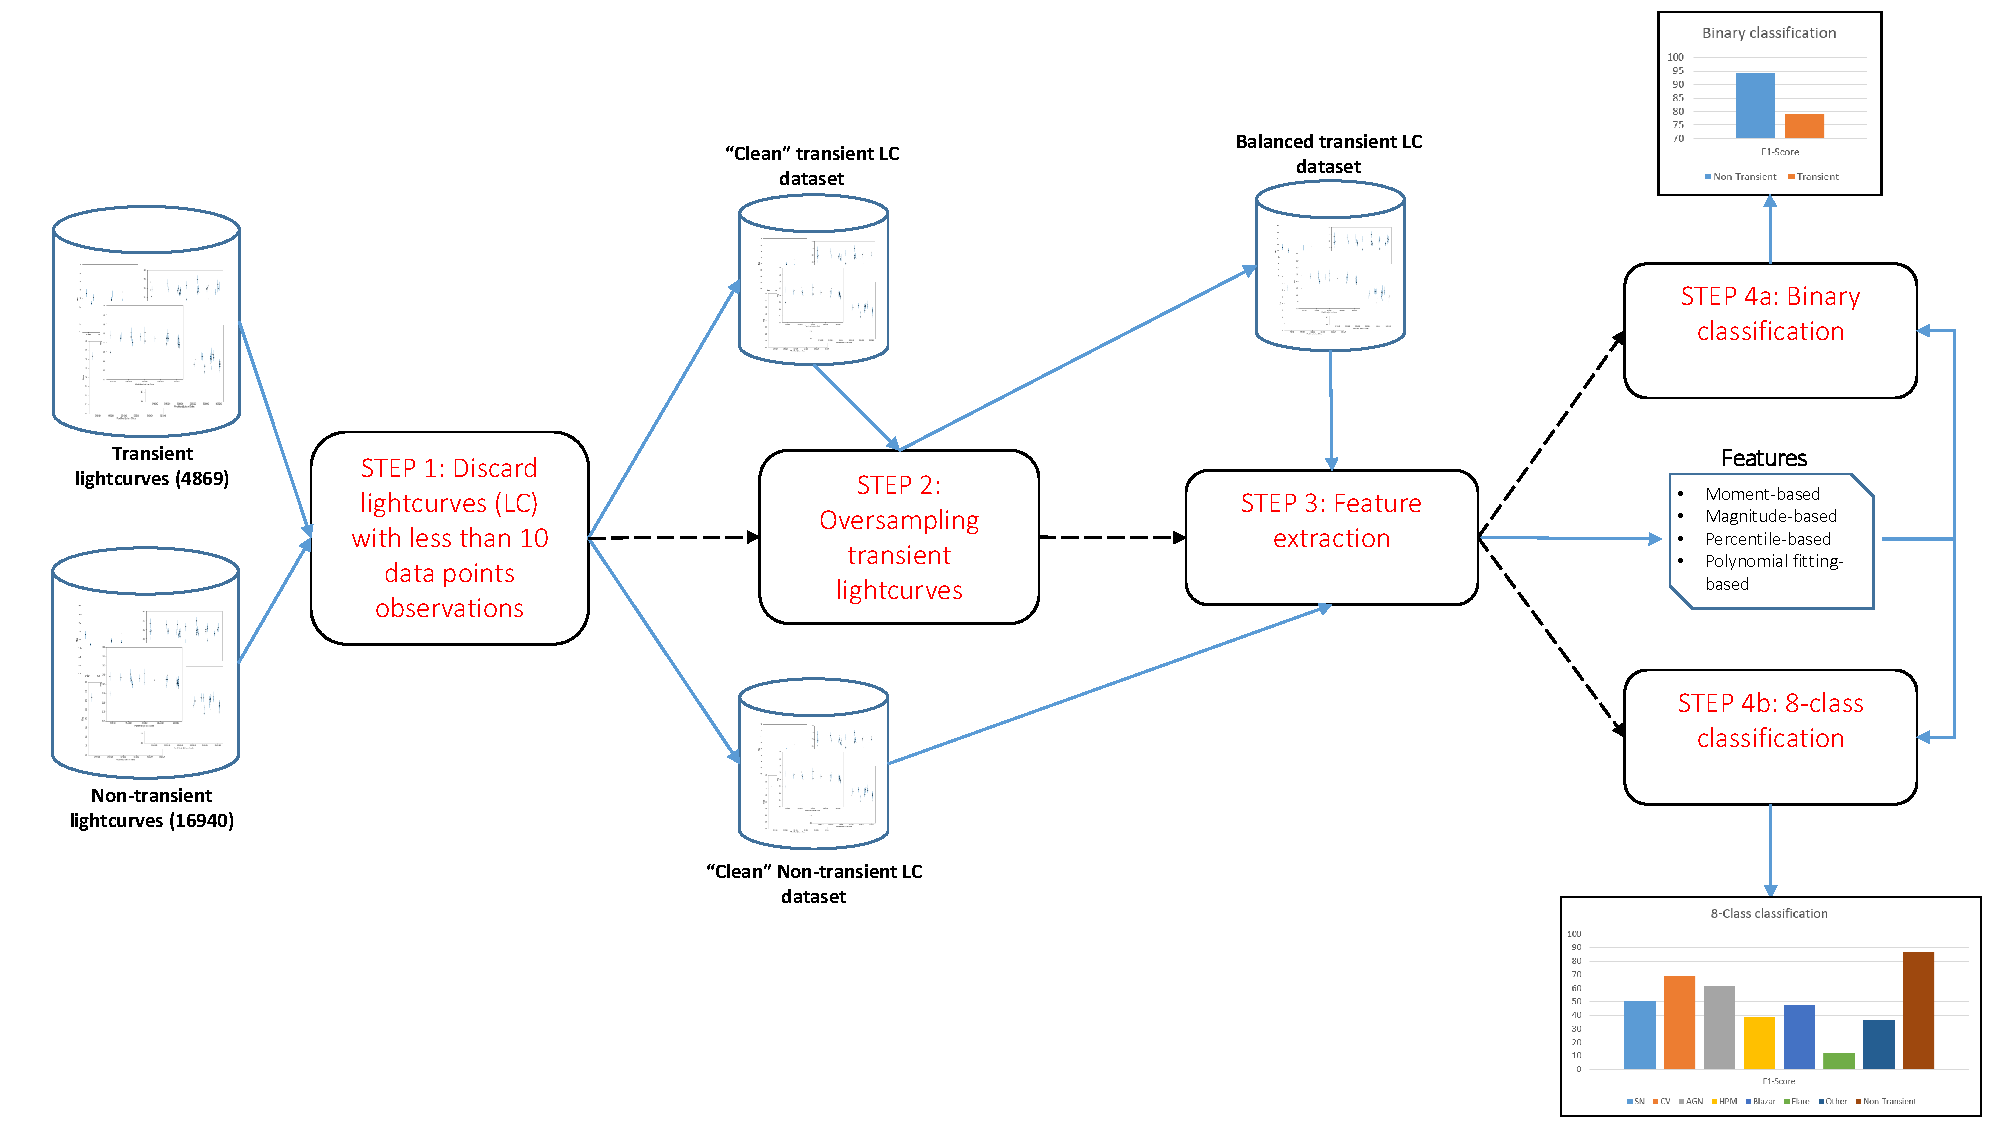
\includegraphics[width=0.9\textwidth]{ML.pdf}
  \caption{Overview of the Machine Learning process on the MANTRA dataset for the binary and 8-class classification tasks. We take the raw lightcurves as input, preprocess the data (step 1) and balance the classes for the training phase (step 2). The final classification (step 4) follows the feature extraction stage (step 3).}
  \label{fig:ML}
\end{figure*} 


Given that the number of lightcurves per class is imbalanced, 
in order to have the same number of instances for each class, we implement an
oversampling step by artificially generating multiple mock lightcurves 
from an observed one. 
We generate a slightly different lightcurve from the observed lightcurve and 
then sample the observed magnitude from a Gaussian distribution
centered on the observational apparent magnitude with the magnitude's
error as the standard deviation. 


Finally, we compute a standard set of features for each lightcurve. 
These features are scalars derived from statistical and model-specific
fitting techniques. 
The first features (moment-based, magnitude-based and
percentile-based) were formally introduced in 
\cite{1101.1959}, and have been used in other studies \citep{1603.00882,1601.03931}.  
We extend that list to include another set (polynomial fitting-based features). 
At the end of this process we normalize the features to have zero
mean and unit variance.  

These groups of features are:

\begin{enumerate}
    
\item Moment-based features, which use the magnitude for each lightcurve.
  \begin{itemize}
  \item \texttt{beyond1std}: 
    Percentage of observations which are over or under one standard
    deviation from the weighted average. Each weight is calculated as
    the inverse of the corresponding observation's photometric error. 
  \item \texttt{kurtosis}: 
    The fourth moment of the data distribution. 
  \item \texttt{skew}: 
    Skewness. Third moment of the data distribution.
  \item \texttt{sk}:
    Small sample kurtosis.
  \item \texttt{std}::
    The standard deviation.
  \item \texttt{stetson\_j}:
    The Welch-Stetson J variability index
    \citep{1996PASP..108..851S}. A robust standard deviation. 
  \item \texttt{stetson\_k}:  The Welch-Stetson K variability index
    \citep{1996PASP..108..851S}. A robust kurtosis measure. 
  \end{itemize}
  
\item Features based on the magnitudes.
    \begin{itemize}
    \item \texttt{amp}: 
      The difference between the maximum and minimum magnitudes.
    \item \texttt{max\_slope}: 
      Maximum absolute slope between two consecutive observations.
    \item \texttt{mad}: 
      The median of the difference between magnitudes and the median
      magnitude. 
    \item \texttt{mbrp}: 
      The percentage of points within 10\% of the median magnitude.
    \item \texttt{pst}: 
      Percentage of all pairs of consecutive magnitude measurements that have positive slope.
    \item \texttt{pst\_last30}: 
      Percentage of the last 30 pairs of consecutive magnitudes that
      have a positive slope, minus percentage of the last 30 pairs of
      consecutive magnitudes with a negative slope. 
    \end{itemize} 


  \item Percentile-based features, which use the sorted flux distribution for
    each source. The flux is computed as $F = 10^{0.4 \mathrm{mag}}$. 
    We define $F_{n,m}$ as the difference between the $m$-th and $n$-the flux
    percentiles. 
    \begin{itemize}
    \item \texttt{p\_amp}: 
      Largest percentage difference between the absolute maximum
      magnitude and the median. 
    \item \texttt{pdfp}: 
      Ratio between $F_{5,95}$ and the median flux.
    \item \texttt{fpr20}: 
      Ratio $F_{40,60} / F_{5,95}$
    \item \texttt{fpr35}:
      Ratio $F_{32.5,67.5} / F_{5,95}$
    \item \texttt{fpr50}: 
      Ratio $F_{25,75} / F_{5,95}$
    \item \texttt{fpr65}: 
      Ratio $F_{17.5,82.5} / F_{5,95}$
    \item \texttt{fpr80}: 
      Ratio $F_{10,90} / F_{5,95}$
    \end{itemize}
    
  \item Polynomial Fitting-based features, which are the coefficients of
    multi-level terms in a polynomial curve fitting. This is a new set
    of features proposed in this paper. 
    \texttt{Polyn\_Tm} indicates the coefficient of the term of order
    \texttt{m} in a fit to a polynomial of order \texttt{n}.
    \begin{itemize}
        \item \texttt{Poly1\_T1}.
        \item \texttt{Poly2\_T1}.
        \item \texttt{Poly2\_T2}.
        \item \texttt{Poly3\_T1}.
        \item \texttt{Poly3\_T2}.
        \item \texttt{Poly3\_T3}.
        \item \texttt{Poly4\_T1}.
        \item \texttt{Poly4\_T2}.
        \item \texttt{Poly4\_T3}.
        \item \texttt{Poly4\_T4}.
    \end{itemize}    
\end{enumerate}


\subsection{ML algorithms}

We conduct experiments with three widely used families of supervised classification 
algorithms \citep{skysurvey, 1601.03931}: Neural Networks (NNs), Random Forests (RFs) and Support
Vector Machines (SVMs). 

These algorithms are popular in published studies and are efficient 
for low dimensional feature datasets as is our case. 
We use sklearn \citep{1201.0490} Python's implementation of random forests and support vector machines. 
Details on the inner workings of these machine learning models can be found in \cite{9780387848570}.

We use the pytorch library for python for the development of the linear neural Networks. It consists of a series of fully connected layers that map the features to the corresponding number of classes. At each layer, a 1d batch normalization is implemented followed by a relu activtion function. The final layer invokes a softmax activation function to transform the numercal values to class probabilities.

The hyperparameters explored for each algorithm are the
following. 

\begin{itemize}
\item Neural Networks:
\begin{itemize}
\item Learning Rate: $\{0.1,0.01,0.001,0.0001\}$
\item Hidden Layer Sizes: Single , double or triple layers with $500$ nodes each.
\end{itemize}

\item Random Forest:
\begin{itemize}
    \item Number of Estimators: $200$ or $700$.
    \item Number of features considered: Square root or $log_2$ of the total number of features.
\end{itemize}

\item Support Vector Machines:
\begin{itemize}
    \item Kernels: Radial Basis Function (RBF), linear or sigmoid.
    \item Kernel Coefficient ($\gamma$):  
      $\{0.125, 2, 32\}$
    \item Error Penalty (\textit{C}): $\{0.125, 2, 32\}$
\end{itemize}
\end{itemize}

\subsection{Validation} \label{subsection_importances}

We split the input lightcurves into training and testing in a $75:25$ ratio respectively, class by class.


For the random forests and the SVM, we use a grid search over the hyperparameter combinations with a 2-fold cross-validation over the training set to determine the best hyperparameters. 

For the neural networks, at each epoch, the network is evaluated on the test data. 
% \begin{figure*}
% 	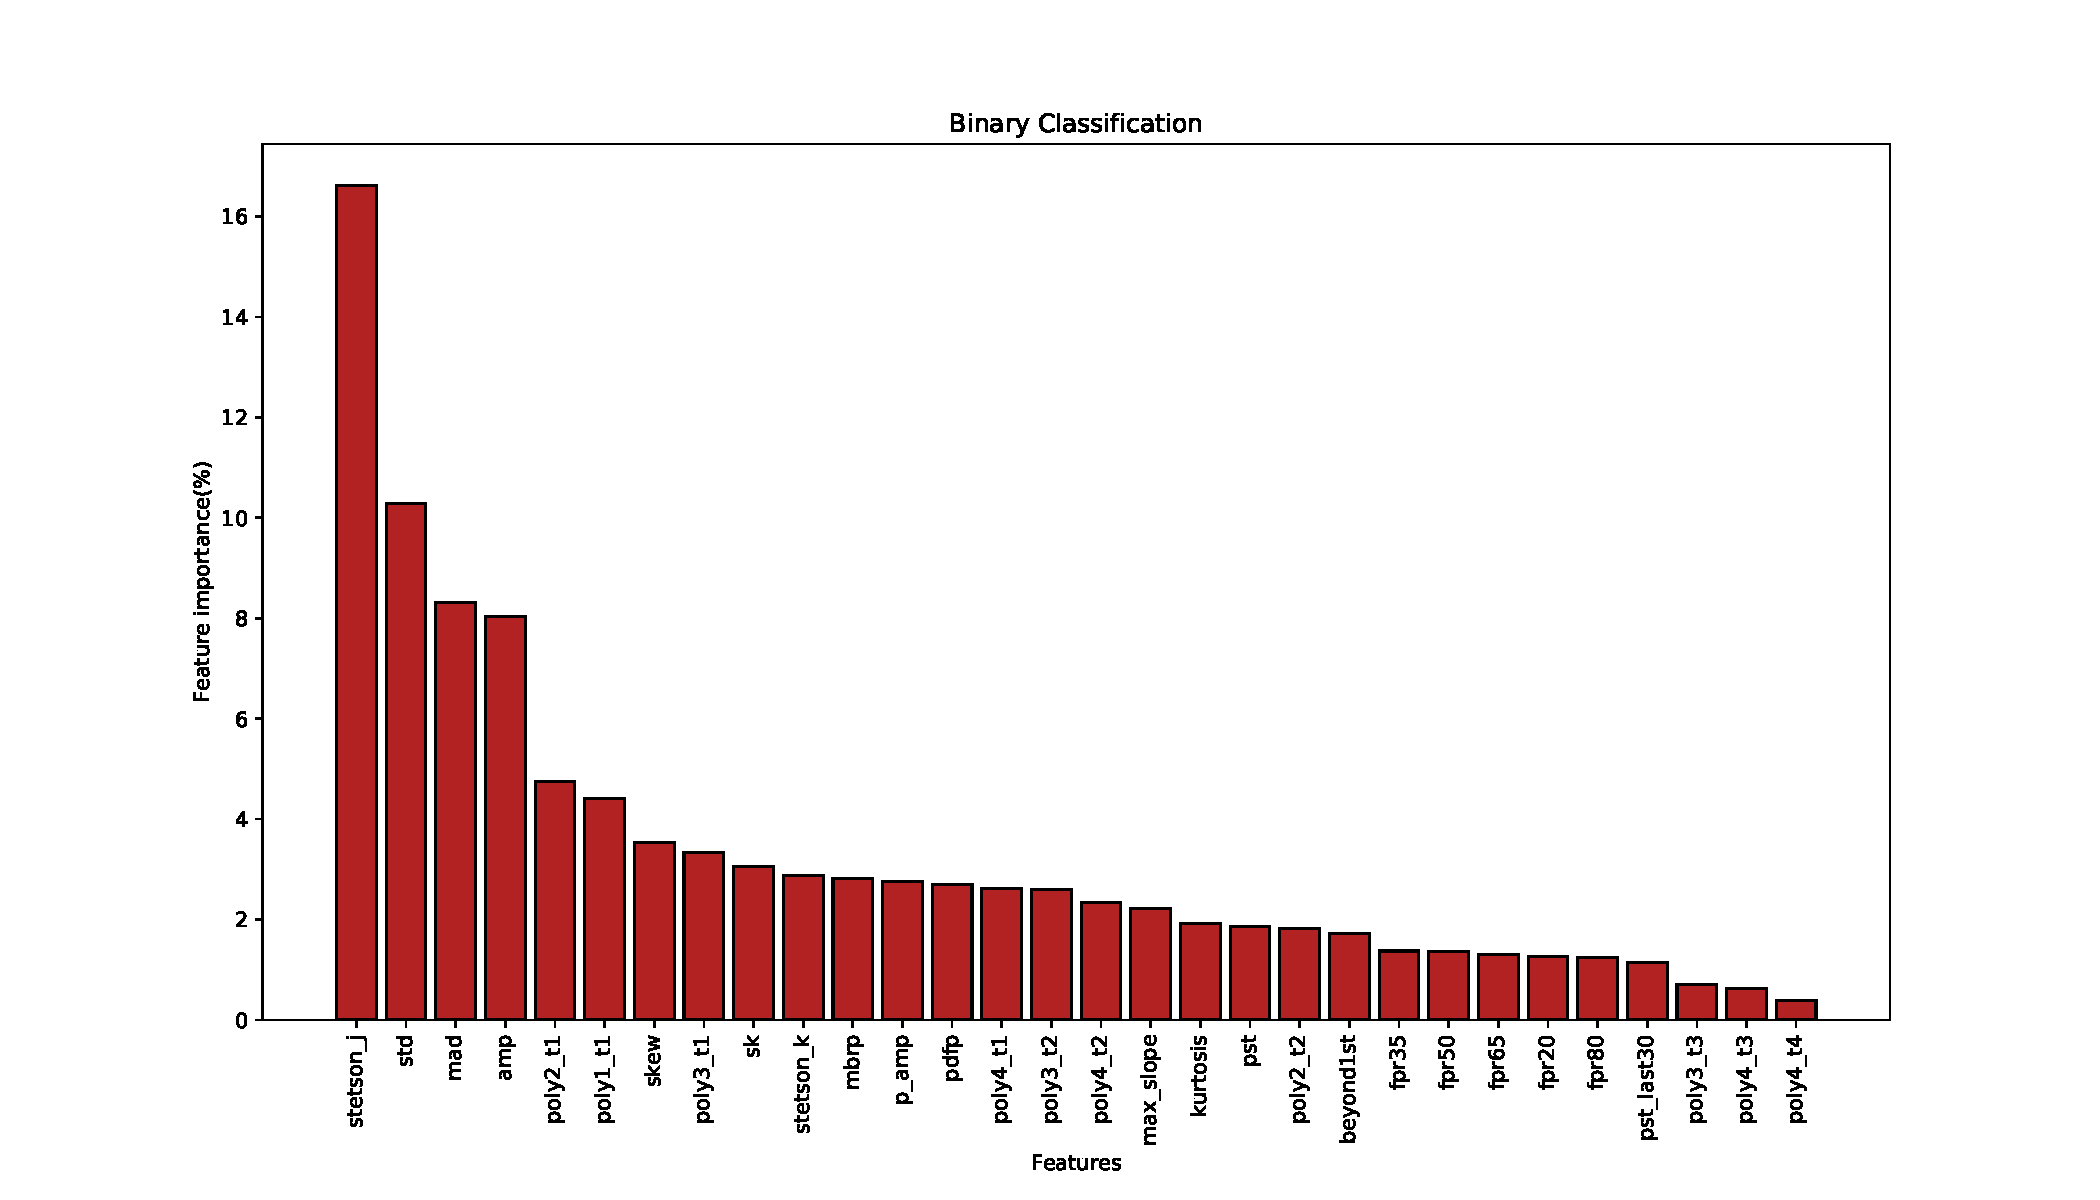
\includegraphics[width=\textwidth]{binFeatImportance.pdf}
%     \caption{Feature importance rank  for the best Random Forest
%       classifier for the Binary classification task. 
%       Feature importance is represented with percentages.} 
%     \label{Importances-Binary}
% \end{figure*} 

% \begin{figure*}
% 	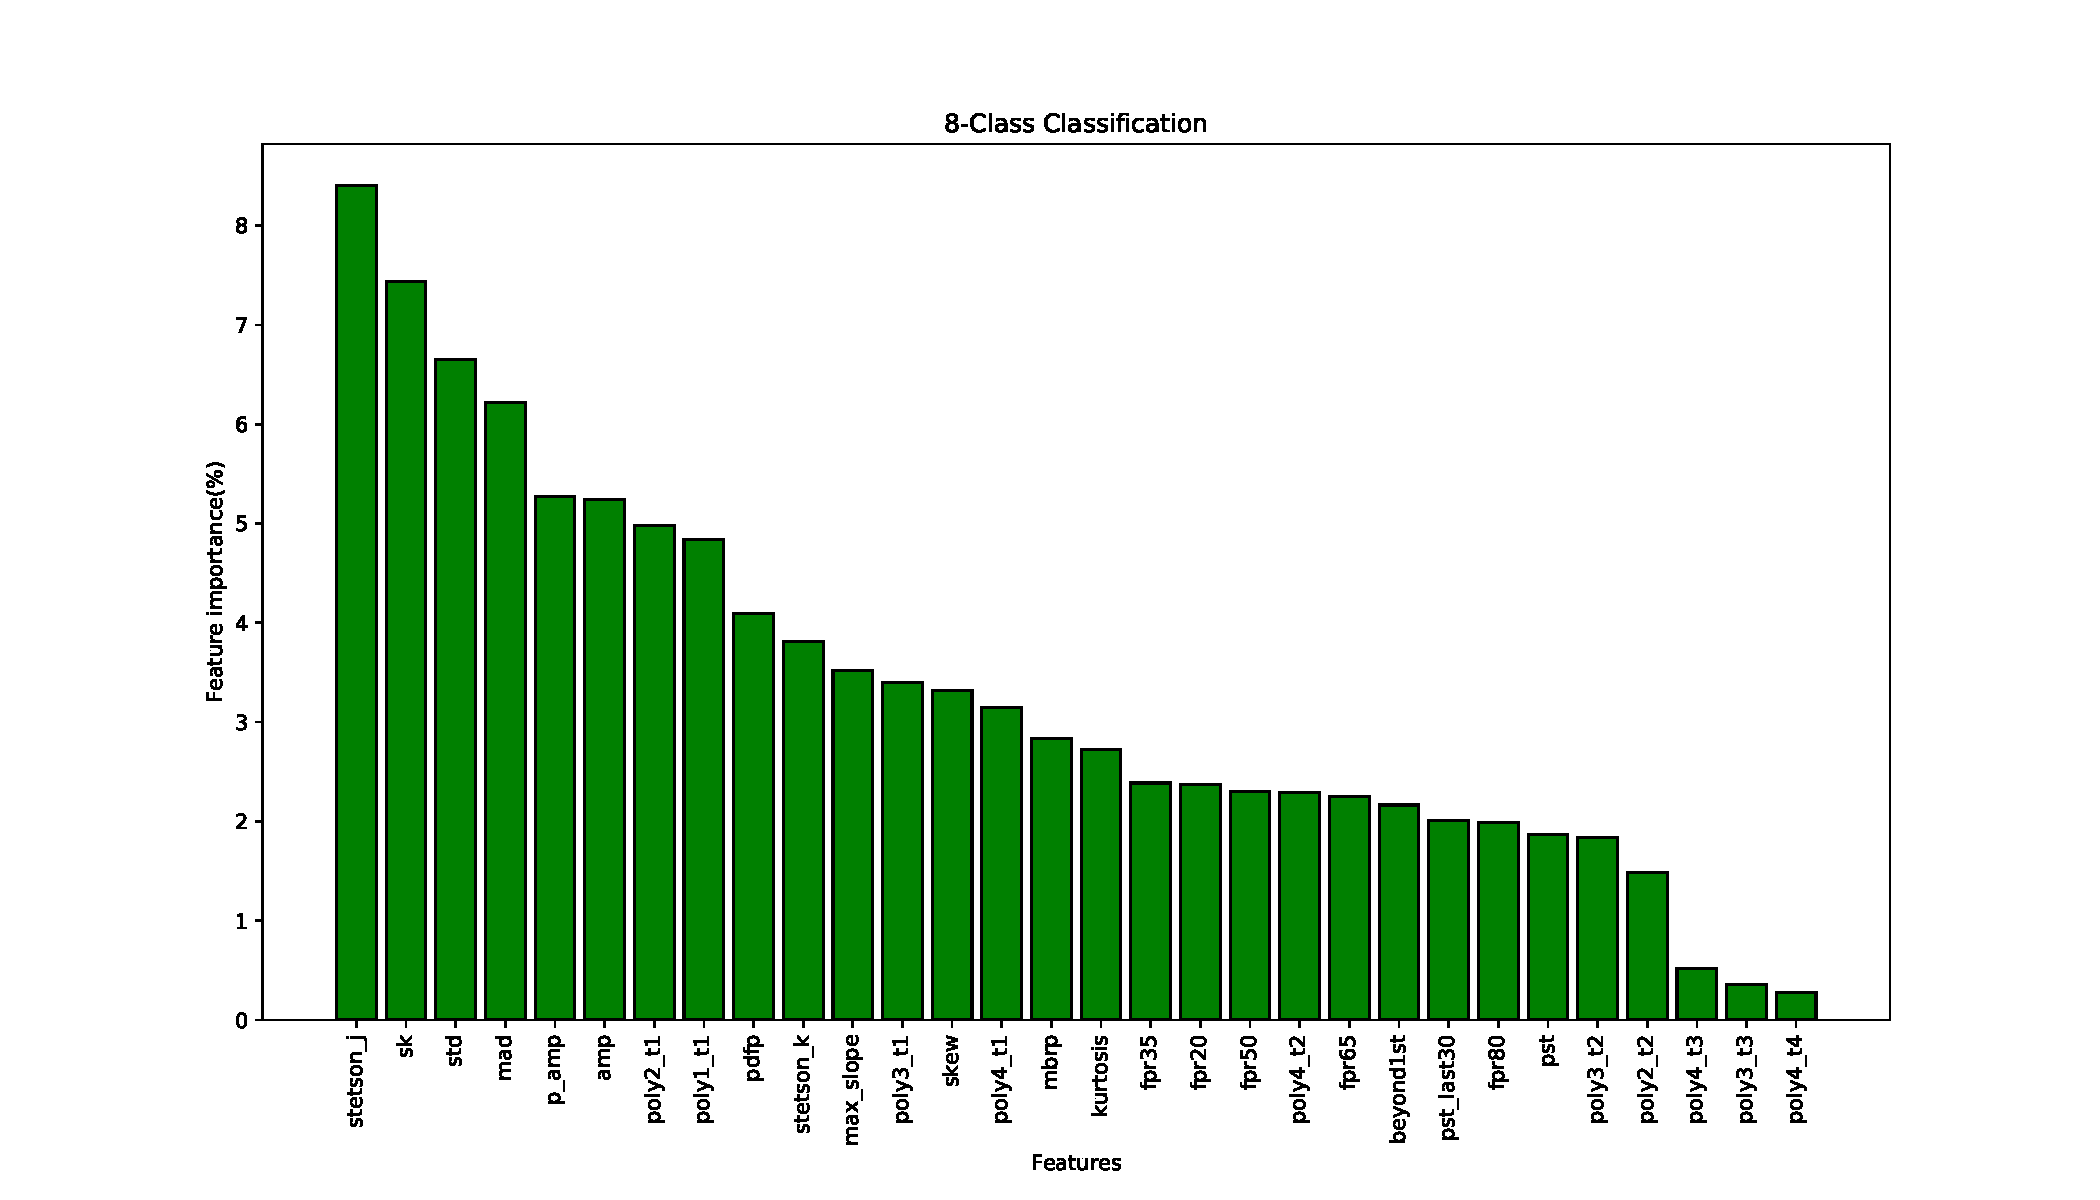
\includegraphics[width=\textwidth]{8classFeatImportance.pdf}
%     \caption{Feature importance rank for the best Random Forest
%       classifier for the best 8-Class classification task. Feature
%       importance is represented with percentages.} 
%     \label{Importances-8-Class}
% \end{figure*}

\subsection{Results}

Table \ref{table:all-avg-results} shows the average class precision, recall and F1-measre for each of the classification tasks and algorithms liste above. 


\begin{table}
\centering
% \resizebox{0.45\textwidth}{!}{%
\begin{tabular}{ccccc}
\hline
\multicolumn{1}{l}{\textbf{Case}} & \textbf{Classifier} & \textbf{Precision} & \textbf{Recall} & \textbf{F1-score} \\ \hline \hline
\multirow{3}{*}{Binary}                 & RF                  & \textbf{86.615}    & \textbf{86.615} & \textbf{86.615}   \\
                                        & SVM                 & 82.615             & 82.525          & 82.57             \\
                                        & NN                  & 71.84              & 73.19           & 72.51             \\ \hline
\multirow{3}{*}{8 Class}                & RF                  & 46.25              & \textbf{63.59}  & 50.38             \\
                                        & SVM                 & 32.94              & 55.22           & 36.60             \\
                                        & NN                  & \textbf{61.86}     & 61.86           & \textbf{61.86}   \\ \hline
\end{tabular}%
% }
\caption{Average precision, recall and F1-score accross all classes for each algorithm and classification task. Best results per metric per classification task are highlighted in bold.}
\label{table:all-avg-results}
\end{table}

%%%%%%  BINARY  %%%%%%
\subsubsection{Binary Classification} 
\label{Results-Binary} 

The best algorithm in this task is RFs with an average F1-Score of
87.69\%.   
SVMs are the second best-performing model with a F1-Score of 85.36\%. 
Changing the number of features does not significantly affect the score.
NNs are ranked third, although their scores are very similar to those of SVMs. 
The highest achieved score for NNs is 85.03\%.

Figure \ref{fig:normalizedBinaryCM} shows the confusion matrix of the best
performing algorithm and Table \ref{Overall-Scores-Binary} summarizes 
the metrics for transient and non-transient class. These results suggest 
that in an imbalanced set up, non-transient sources are better classified, 
while transients are more difficult, showing a difference of about 
14 points in F1-Score compared to the non-transient class. 
This difference in performance could be attributed to the intra-class
variation within the transient class because of the different 
types of transient sources.  

Figure \ref{Importances-Binary} displays the most important features
for the RFs classifier.
The top five inputs for classification are \texttt{stetson\_j},
\texttt{std}, \texttt{mad}, \texttt{poly1\_t1} and \texttt{poly2\_t1}.  
The first feature achieved the highest importance of 21\%, compared to
the following with values in the range 6\% - 8\%.  


\begin{table}
\centering
\begin{tabular}{|r|c|c|c|c|}
\hline
\multicolumn{1}{|l|}{} & Precision & Recall & F1-Score & No. instances \\ \hline \hline
Non-Transient          & 94.13     & 94.13      & 94.13      & 3798   \\ \hline
Transient              & 79.10     & 79.10      & 79.10      & 1067    \\ \hline
\end{tabular}
\caption{Precision, Recall and F1-Score for the Binary Classification Task.}
\label{Overall-Scores-Binary}
\end{table}


\begin{figure}
\begin{center}
	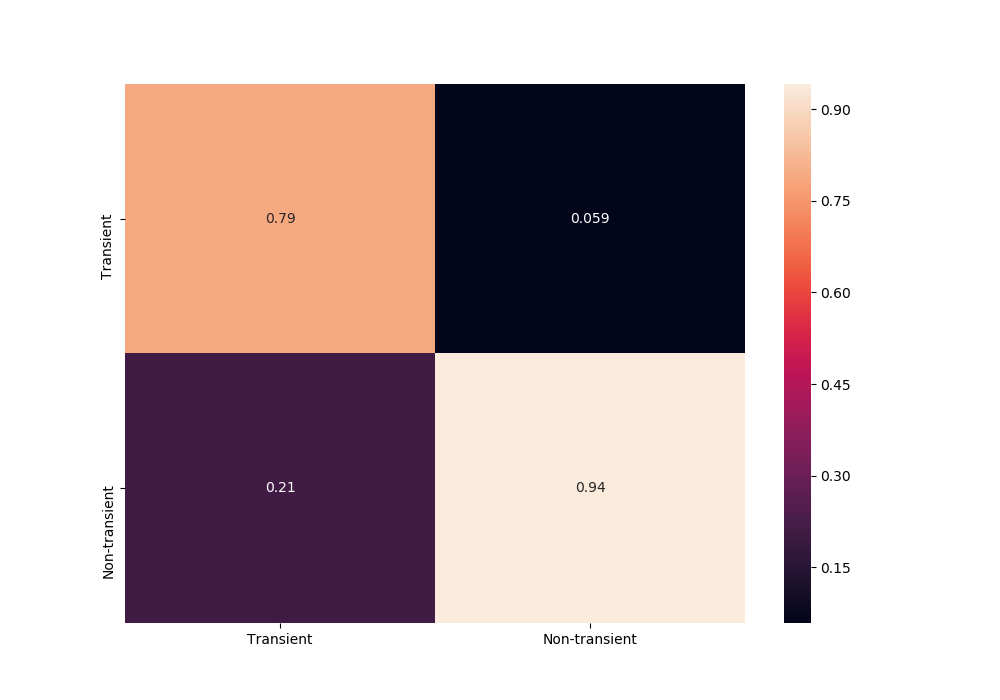
\includegraphics[width=0.6\textwidth]{normalizedCMBinary.png}
\end{center}
  \caption{Confusion Matrix for the best performing model in the Binary task. Rows represent prediction and columns the ground truth.}
  \label{fig:normalizedBinaryCM}
\end{figure} 





%%%%%%  EIGHT-CLASS  %%%%%%
\subsubsection{Eight-Class Classification}

For this task, RFs are again the best classifier.  
The best F1-Score is 66.05\%. 
NNs are the second best model. 
Their highest F1-Score is 60.19\%, while SVMs are the worst-performing
model only achieving an average F1-Score of 57.30\%.
Table \ref{Overall-Scores-8-Class-Regular} summarizes the results for 
individual classes and Table \ref{Confusion-8-Class} presents 
the confusion matrix for the RFs.

The two classes with highest F1-Score are non-transient (87.12\%) and CV (68.77\%). 
The recall decreases for the non-transient class in comparison to the binary experiment, 
meaning that the algorithm misclassified some instances that belong to non-transient class
among transient classes. 
However, transient sources are not commonly confused with non-transient ones. 
The worst performing classes are Flare, Other and HPM, with F1-Scores in the 
range 11\% - 40\%. 
It is worth noting that the less frequent classes present a lower performance, 
such as Flare and HPM. 
Even though the most frequent classes are more easily identified, 
the "other" type class has a low F1-score due to the different nature 
of sources that were assigned to this category. 


SN is the class with which most other class instances are
incorrectly classified. 
Moreover, Flares have about 50\% of the test samples classified as
non-transients, AGNs have about 20\% of their 
samples classified as Other, and Blazars and Other had most of  its
samples classified as AGN. 
Additionally, most incorrectly classified AGNs ($\sim$20.5\%) are
identified as Other, and most Blazar instances are
incorrectly categorized as either SN or AGN. 


Figure \ref{Importances-8-Class} displays the feature importance ranking.
This list ranks first \texttt{stetson\_j} with an 8\% importance,
followed by \texttt{amp}, \texttt{sk}, \texttt{std}, \texttt{mad},
with values around 6\%.   

\begin{table}
\centering
% \resizebox{\textwidth}{!}{%
\begin{tabular}{cccc}
\hline
\textbf{Class} & \textbf{Precision} & \textbf{Recall} & \textbf{F1-score} \\\hline \hline
SN             & 34.89              & 34.67           & 34.78             \\\hline
CV             & 61.86              & 61.86           & 61.86             \\\hline
AGN            & 34.84              & 72.64           & 47.09             \\\hline
HPM            & 11.90              & 85.52           & 20.90             \\\hline
Blazar         & 26.78              & 50.84           & 35.08             \\\hline
Flare          & 5.25               & 43.13           & 9.36              \\\hline
Other          & 18.26              & 26.06           & 21.47             \\\hline
Non-Tr.        & 94.20              & 66.82           & 78.18             \\\hline
avg/total      & 61.86              & 61.86           & 61.86             \\\hline
\end{tabular}%
\caption{Precision, Recall and F1-Score for the 8-Class Classification Task.}
\label{Overall-Scores-8-Class-Regular}
% }
\end{table}


\begin{figure}
\begin{center}
	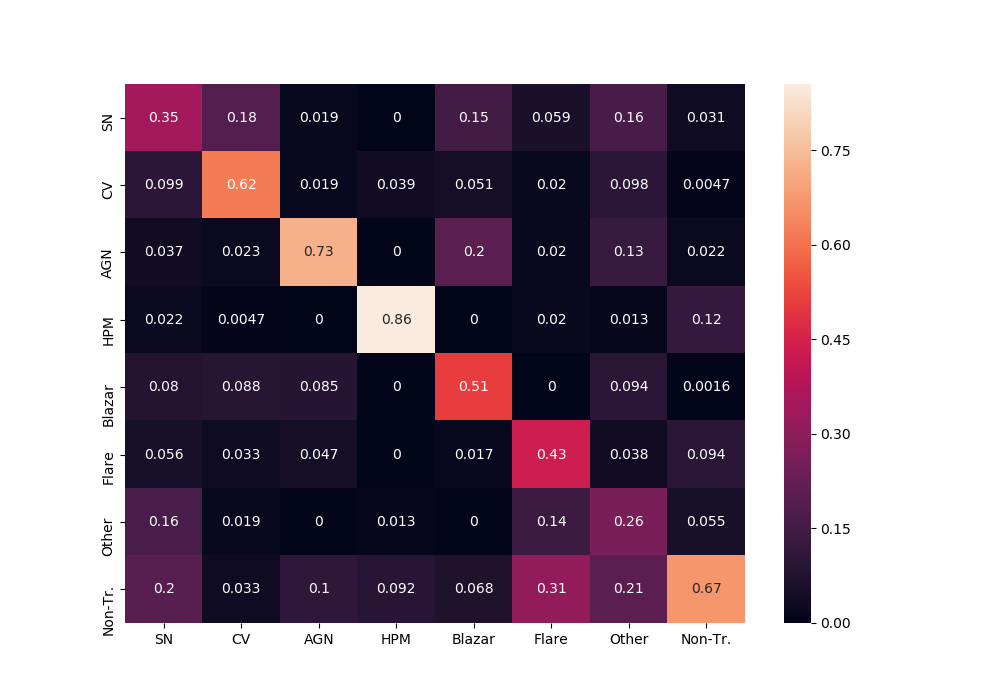
\includegraphics[width=0.8\textwidth]{normalizedCM.png}
\end{center}
  \caption{Confusion Matrix for the best performing model in the 8-class
  task. The classes follow the abbreviations in Table \ref{Overall-Scores-8-Class-Regular}. Rows represent the predictions, and columns the ground truth.}
  \label{fig:normalized8ClassCM}
\end{figure} 


\section{Conclusions}
\label{sec:conclusions}

The scope of forthcoming large astronomical synoptic surveys 
motivates the development and exploration of automatized ways to
detect transient sources. 
In turn, this need prompts the compilation of publicly available databases
to train and test new algorithms. 
In this paper we presented the results of such a compilation based on data
from the Catalina Real-Time Transient Survey.
The data-set compiles  $4869$ transient and $16940$ non-transient
lightcurves. 
The dataset is publicly available at
\url{https://github.com/MachineLearningUniandes/MANTRA}.   

We illustrated how to use this database by extracting 
characteristic features to use them as input to train three different
machine learning algorithms (Random Forests, Neural Networks and
Support Vector Machines) for classification tasks.
The features extracted from lightcurves were either statistical
descriptors of the observations, or polynomial curve fitting
coefficients applied to the lightcurves.   
Overall, the best classifier for all tasks was the Random Forest.
In this model the most important feature was always
\texttt{stetson$\_$j}, i.e. a robust estimate for the standard
deviation. 

In a second paper we will present another reference dataset for
astronomical transient event recognition based on images of the
CRTS.
The corresponding tests will use  state-of-the art deep learning
techniques for transient classification. 

\section*{Acknowledgements}

We thank Andrew Drake for sharing with us the CRTS Transient dataset
used in this project.  
We acknowledge funding from Universidad de los Andes in the call for
project finalization.
We also thank contributors and collaborators of the SciKit-Learn,
Jupiter Notebooks and Pandas' Python libraries.  

CRTS and CSDR2 are supported by the U.S.~National Science 
Foundation under grant NSF grants AST-1313422, AST-1413600, and 
AST-1518308.  The CSS survey is funded by the National Aeronautics
and Space Administration under Grant No. NNG05GF22G issued through
the Science Mission Directorate Near-Earth Objects Observations Program.

\bibliographystyle{mnras}
\bibliography{bibliography}

\end{document}

